\documentclass{article}
\usepackage{amsmath, amssymb, amsthm}
\usepackage[pdftex]{graphicx}
\usepackage{slashbox, booktabs}
\usepackage{pdflscape}

\title{Project 3}
\author{Ni, Angxiu}
\date{April, 2014}

\begin{document}
\maketitle

\section{Answer questions}
\label{sec: Q1}
This document is only a template.
\subsection{Derive the adjoint system}
The primal problem is to find $u, \bar{F}$, s.t., $\forall w, \lambda,$
    \[ R(u, \bar{F}, w, \lambda) = \langle w, \bar{F}\rangle  +\langle \lambda, u-g\rangle  - (w', cu-\nu u') + (w, bu-f) = 0 \]
    \[ \Leftrightarrow a (u, \bar{F}, w, \lambda) = l(w,\lambda) \]
And evaluate the objective by,
    \[ J = l^o (u ,\bar{F}) \]
Here,
    \[ a(u, \bar{F}, w, \lambda) = \langle w, \bar{F}\rangle  +\langle \lambda, u\rangle  - (w', cu-\nu u') + (w, bu) = 0 \]
    \[ l(w,\lambda) = (w,f) + \langle \lambda, g\rangle  \]
    \[ l^o(u, \bar{F}) = cu-\bar{F} = \langle h,u\rangle  +\langle k, \bar{F}\rangle   \]
    \[ g, h, k: \{0, 1\} \rightarrow \mathbb{R} \]
    \[ g(0) = 0, g(1) = 1, h(0)=0, h(1) =c, k(0) = 0, k(1) = -1 \]

The adjoint problem is to find $\psi, \Phi$, s.t., $\forall w, \lambda:$
    \[ a (w, \lambda, \psi, \Phi) = l^o (w,\lambda) \]
    \[ \Leftrightarrow \langle \psi, \lambda\rangle  + \langle \Phi, w\rangle  - (\psi', cw-\nu w') + (\psi, bw) = \langle h,w\rangle  +\langle k, \Phi\rangle \]
    \[ \Leftrightarrow \langle \psi, \lambda\rangle  + \langle \Phi+ \nu \psi', w\rangle  + (-\nu \psi'' - c\psi'+b\psi, w) = \langle h,w\rangle  +\langle k, \Phi\rangle \]
    \[ 
    \Rightarrow \left\{ \begin{array}{rcl}
    -\nu \psi'' - c\psi'+b\psi =0  & on & [0,1] \\
    \psi=k& at &\{0,1\} \\
    \Phi + \nu \psi'=h& at &\{0,1\} 
    \end{array}\right. 
    \]
The objective is now evaluated by,
    \[ J = l (\psi ,\Phi) =  (\psi,f) + \langle \Phi, g\rangle  \]
    
\subsection{Check consistency}
Now denote the discrete bilinear form by $a_{hp}$, and the continuous version is denoted by $a$. Since for the exact $\psi$ is smooth, all jumps terms in $\psi$ vanishes, and $\{ \psi\} = \psi	$, we just need to prove that,
    \[
    a_{hp}(w_{hp}, \lambda_{hp},\psi,\Phi)  = l^o (w_{hp},\lambda_{hp})
    \]
    \[
    \Leftrightarrow \langle \psi, \lambda_{hp}\rangle  + \langle \Phi, w_{hp}\rangle  - (\psi', cw_{hp}-\nu w_{hp}') + (\psi, bw_{hp}) - \sum[w_{hp}]\nu \psi' = <h,w_{hp}> + <k,\lambda_{hp}> 
    \]
    \[
    \Leftrightarrow  \langle \psi, \lambda_{hp}\rangle  + \langle -\nu\psi', w_{hp}\rangle  - (\psi', cw_{hp}-\nu w_{hp}') + (\psi, bw_{hp}) - \sum[w_{hp}]\nu \psi' = <k,\lambda_{hp}>
    \]
    \[
    \Leftrightarrow  \langle -\nu\psi', w_{hp}\rangle  - (\psi', cw_{hp}-\nu w_{hp}') + (\psi, bw_{hp}) - \sum[w_{hp}]\nu \psi' = 0
    \]
    \[
    \Leftrightarrow  - (\psi', cw_{hp}-\nu w_{hp}') + (\psi, bw_{hp}) - \sum <w_{hp},\nu \psi'>_\kappa = 0
    \]
    \[
    \Leftrightarrow  - (\psi', cw_{hp}) + (\psi, bw_{hp}) - \sum (w_{hp}, \nu \psi'')_\kappa = 0
    \]
    \[
    \Leftrightarrow  (-\nu \psi'' -c\psi' +b\psi, w_{hp}) = 0
    \]
This last equality is true, due to the governing PDE for $\psi$.

\section{Solve the adjoint problem}
\label{sec:adjoint solve}
\subsection{ Numerical solution of $u_{hp}$ and $\psi_{hp}$}
Both primal and adjoint problem are solved by the code submitted. 
Just to give an idea of how the solution looks like, 
$u_{hp}$ and $\psi_{hp}$ solved using p=3 and mesh number 128 is shown below:
\begin{center}
	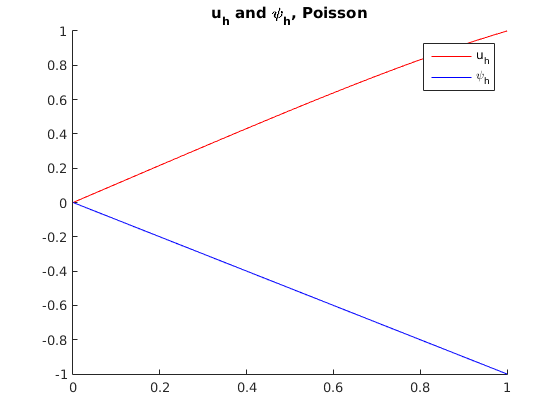
\includegraphics[scale = 0.8] {upsiP.png}
\end{center}

\end{document}
